\documentclass[12pt,letterpaper,reqno]{amsart}
\usepackage{enumerate}
\usepackage[shortlabels]{enumitem}
\usepackage{graphicx}
\usepackage{amssymb}
\usepackage[normalem]{ulem}
\usepackage{titlesec,bbm, hyperref}
\usepackage{spverbatim} 
\usepackage{tikz}
\usepackage{caption}
\usepackage{subcaption}
\usepackage{geometry}
\geometry{letterpaper, portrait, margin=0.5in}

\newcommand{\R}{\mathbb R}
\newcommand{\Q}{\mathbb Q}
\newcommand{\N}{\mathbb N}
\newcommand{\norm}[1]{\left\vert #1 \right \vert}	
\newcommand{\Norm}[1]{\left\Vert #1 \right \Vert}
\renewcommand{\span}{\operatorname{span}}


\begin{document}

\thispagestyle{empty}
\centerline{\Large Math 675 Homework 9}
\centerline{Sumanth Ravipati - 11/7/2018}
\vspace{.25in}

\begin{enumerate}[1.]
\item Is the completion of an inner product space a Hilbert space? Explain.\newline
\begin{flushleft}
Yes, as a Hilbert space ($H$) is simply a complete inner product space, we can add the limits of an inner product space ($I$)'s Cauchy sequences to the space. To prove this, let us consider the collection of all Cauchy sequences $\{f_n\}$ with $f_n \in I$. Let us define an equivalence relation $\sim$ in this collection as follows: $\{f_n\} \sim \{f_m\}$ if $f_n - f_m$ converges to 0 as $n \rightarrow \infty$. We can consider the collection of equivalence classes to be $H$ with an inner product defined as $\lim_{n\rightarrow\infty}(f_n,g_n)$, where $\{f_n\}$ and $\{g_n\}$ are Cauchy sequences in $I$ that represent the elements $f$ and $g$ in $H$. The sequence $\{f_n\} = f \, \forall n$ shows that $I \subset H$. To show that $H$ is a completion of $I$, take the Cauchy sequence $\left\{\{f_n^k\}_{n=1}^\infty\right\}_{k=1}^\infty$, which converges to the limit $F \in H$. The limit can be represented as $\{f^n_{N(n)}\}$, where $N(n)$ is defined as $\left| f _ { N ( n ) } ^ { n } - f _ { j } ^ { n } \right| \leq 1/n$ for $j \geq N(n)$. We then see that $\left\{\{f_n^k\}_{n=1}^\infty\right\}$ converges to $F \in H$, as desired. $\Box$
\newline
\end{flushleft}
\item (Section 15, p.141, Problem 2) Prove each of the following:
\begin{enumerate}
\item Given a Banach space $V$, let $\{B_n\}$ be a nested sequence of closed spheres in $V$. Prove that $\cap_n B_n$ is nonempty. (Note that the radius is not assumed to go to zero, and the centers are not assumed to be the same.)\newline
\begin{flushleft}
Lemma: If $B_r(x) \subset B_s(y)$, then $\Norm{y - x} \leq s - r$. Proof: The 2D projections of the nested spheres will fall under 1 of the 2 situations below:\vspace{1.75in}
\newline
In either case, we see that $\Norm{y - x} + r + b = s$. Since $b \geq 0$, we see that $\Norm{y - x} \leq s - r$.
Suppose $r _ { n } \rightarrow r > 0 .$ Then there is $N$ such that $r _ { N } \leq 2 r$. Then for all $n \geq N$ we have $r \leq r _ { n } \leq r _ { N } \leq 2 r ,$ so $r _ { N } - r _ { n } \leq r$ and the claim implies that $\left\| x _ { n } - x _ { N } \right\| \leq r \leq r _ { n } ,$ so $x _ { N } \in \bigcap _ { n = 1 } ^ { \infty } B _ { \leq r _ { n } } \left( x _ { n } \right)$. Therefore, $\cap_n B_n$ is nonempty, as desired. $\Box$\newline
\end{flushleft}
\item Give an example of a nested sequence of closed non-empty sets $C_i$ in $\R$ such that $\cap C_i=\emptyset$.\newline
\begin{flushleft}
Each term of the sequence $C_i = [i,\infty)$ is closed and non-empty, yet $\bigcap C_i = \emptyset$. This is because for any number $j \in \R$, the intersection $\bigcap\limits_{i=0}^{j+1} C_i$ will exclude $j$.\newline
\end{flushleft}
\item Give an example of a nested sequence $\{E_n\}$ of nonempty closed bounded convex sets in a Banach space $V$ (of your choice) such that $\cap_n E_n=\emptyset$.\newline
\begin{flushleft}
Consider $c_0$ with the supremum norm, and $E_n = \left\{ x \in c _ { 0 } : \| x \| \leq 1 , \sum _ { k = 1 } ^ { \infty } 2 ^ { - k } x _ { k } \geq 1 - 1 / n \right\}$. This is a nested sequence of nonempty closed convex sets. Yet, $\bigcap E_n$ is empty, since the only element it could conceivably contain, $(1,1,1,\ldots)$ is not in $c_0$.\newline
\end{flushleft}
\end{enumerate}
\newpage
\item Let $\{e_i\}$ be an orthonormal basis for a Hilbert space $H$. Take $x_n=e_{2n}$ and $y_n=e_{2n}+\frac{e_{2n+1}}{n+1}$, and set $M=\span(\{x_n\})$, $N=\span(\{y_n\})$. Show that $M+N$ is not closed, even though $M$ and $N$ are both closed.\newline
\begin{flushleft}
Let us define the vector $z = x + y$, where $x \in M$ and $y \in N$. Therefore $z = \sum a_n x_n + \sum b_n y_n$. If we take $\langle z, e_{2n+1}\rangle$, we get $\langle \sum a_n x_n + \sum b_n y_n, e_{2n+1}\rangle = \sum \langle a_n x_n, e_{2n+1}\rangle + \sum \langle b_n y_n, e_{2n+1}\rangle = \sum \langle a_n e_{2n}, e_{2n+1}\rangle + \sum \langle b_n e_{2n}, e_{2n+1}\rangle + \sum \langle b_n\frac{e_{2n+1}}{n+1}, e_{2n+1}\rangle = \sum \langle b_n\frac{e_{2n+1}}{n+1}, e_{2n+1}\rangle = \frac{b_n}{n+1}$. We can then see that the vector $v = \sum \frac{e_{2n+1}}{n+1}$ can only be expressed as $\sum y_n$, which does not converge. Therefore $v \in H$ but $M + N$ does not contain $v$ and so $M + N$ is not closed. $\Box$
\newline
\end{flushleft}
\item Let $f(x)$ be the GDP of Russia between 1990 and 2015, where we take $x\in [0,1]$ with $x=0$ corresponding to 1990 and $x=1$ corresponding to 2015. Approximate $f(x)$ using the cosine Fourier series. How many terms do you need to get a decent approximation? Provide some illustrations. (You will need Mathematica which is available on campus computers and the attached Mathematica file for this. You don't need to know anything about Mathematica, however.)\newline
\begin{flushleft}
As we see below, one gets a decent approximation after 18 terms of the cosine Fourier series. The GDP dip corresponding to the Great Recession only shows up after 15 or so terms. The global minimum and maximum were accurately predicted relatively quickly. The equations below the graphs are the approximations with the first few Fourier coefficients.
\end{flushleft}
\begin{figure}[h]
\centering
\begin{subfigure}{.33\textwidth}
  \centering
  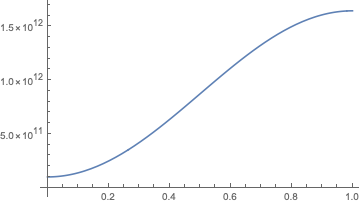
\includegraphics[width=.8\linewidth]{./RussiaGDPn1.png}
  \caption*{$n=1$}
\end{subfigure}%
\begin{subfigure}{.33\textwidth}
  \centering
  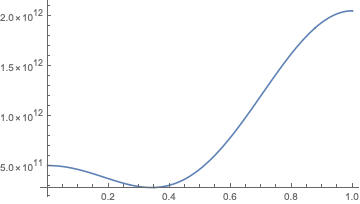
\includegraphics[width=.8\linewidth]{./RussiaGDPn2.png}
  \caption*{$n=2$}
\end{subfigure}
\begin{subfigure}{.33\textwidth}
  \centering
  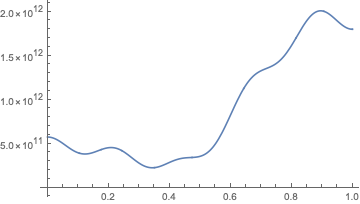
\includegraphics[width=.8\linewidth]{./RussiaGDPn9.png}
  \caption*{$n=9$}
\end{subfigure}
\end{figure}

\begin{figure}[h]
\centering
\begin{subfigure}{.33\textwidth}
  \centering
  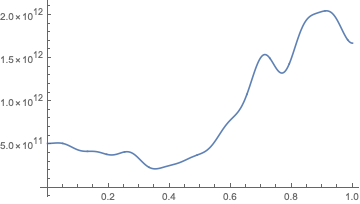
\includegraphics[width=.8\linewidth]{./RussiaGDPn18.png}
  \caption*{$n=18$}
\end{subfigure}%
\begin{subfigure}{.33\textwidth}
  \centering
  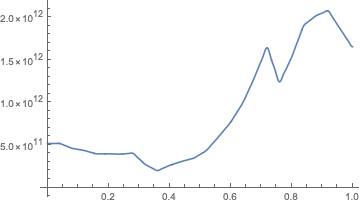
\includegraphics[width=.8\linewidth]{./RussiaGDPn100.png}
  \caption*{$n=100$}
\end{subfigure}
\begin{subfigure}{.33\textwidth}
  \centering
  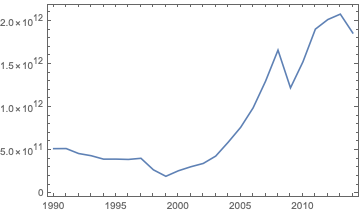
\includegraphics[width=.8\linewidth]{./RussiaGDP.png}
  \caption*{Actual GDP of Russia}
\end{subfigure}
\end{figure}
\begin{flushleft}
$n=1: 8.72101\times 10^{11}-7.73342\times 10^{11} \cos (\pi  x)$\newline
$n=2: 8.72101\times 10^{11}-7.73342\times 10^{11} \cos (\pi  x)+4.04172\times 10^{11} \cos (2 \pi  x)$
$n=9: 8.72101\times 10^{11} -7.73342\times 10^{11} \cos (\pi  x)+4.04172\times 10^{11} \cos (2 \pi  x)+4.63147\times 10^{10} \cos (3 \pi  x)-6.87921\times 10^{10} \cos (4 \pi  x)+2.26595\times 10^9 \cos (5 \pi  x)+1.16897\times 10^{10} \cos (6 \pi  x)+2.63286\times 10^{10} \cos (7 \pi  x)-3.31438\times 10^{10} \cos (8 \pi  x)+8.62262\times 10^{10} \cos (9 \pi  x)$
\end{flushleft}
\end{enumerate}
\end{document}